\documentclass{ctexart}
\usepackage[hmargin=1.1in,vmargin=1in]{geometry}
\usepackage{graphicx}

\title{《信号处理导论》课程报告一}
\input{personal_info/info.tex}

\begin{document}
    \maketitle

    \section{我学到了哪个知识点?}

    信号的概念。在课程的绪论部分,我学到了信号是信息的载体,是信息的物理体现,\textbf{一般是随时间或者位置变化的物理量},
    并且既能按照实际用途分类,也能\textbf{按照时间特性(数学特征)分类}。

    信号可表示为关于时间的函数。

    来源:《信号与线性系统分析》第四版——吴大正 1.2 节 信号。

    \section{我之前是怎么想的?}

    信号是一种事件,或者说,“一种实体”,用来传达某一事件有所发生,比如说红灯亮,红绿灯发出的光信号传达“红灯亮了”这一事件
    的发生。信号只能按照其介质分类,即光信号、电信号、声信号(机械波信号)等等。

    \section{我之前的想法怎么样?}

    以偏概全的错误想法。按照我之前的定义,信号本身作为一种事件,仅存在于某个无限小的时间点上,因此单个信号只能传递 1 比特
    的信息,也不支持如去杂等处理操作。信号可以用关于时间 $t$ 的函数 $f(t)$ 来表示,而我之前的想法则是将函数在某一点的取
    值 $f(t) | _{t=t_0}$ 当作了信号本身,从而使得信号无法被作为数学对象来研究,也无法被以各种手段进行处理,甚至连信号
    的时间特性(比如,红灯在 $t=t_0$ 到 $t=t_1$ 这段时间内亮)这样信号的基本属性都无法解释。

    \section{我应该怎样想才对?}

    信号是一个物理量,其存在与否与事件是否发生无任何关系,信号无需为“事件”负责。用回到刚才的例子,对于某一盏红绿灯 $A$,
    只要这盏灯存在,那么不管它在某一时刻到底是什么状态,“红绿灯 $A$ 的红灯亮不亮”,或者“红绿灯 $A$ 是什么状态”这些信号
    就一直存在,“红灯亮”这个事件只能表明,在这个事件发生的那一个时刻,或者一段时间间隔内,上述信号的取值发生了改变(具体
    取值或者编码如何是另一个话题),而不是“这个事件导致了信号的产生”。

    \section{我应该怎样用上它?}

    信号本身作为一个函数,可以携带大量的信息。那么,我们能不能在传递信号的时候,不是直接传递信号随时间的取值,而是传递信号
    与时间的表达式,从而减小传递信号所需要的资源(比如,记录某段时间内某江面水位的高低,记录一个函数表达式而不是这一段时间
    内每次监测时水位的高低)并且减小信号被干扰的可能性?

    信号本身作为一个函数,是“被动实体”不会“主动”修改自己,那么信号的失真必然是由于传递信号的系统对信号产生了某种作用,而
    提高信号的“保真度”就要靠减小传递系统对信号产生这种“作用”的可能性。

    \section*{字数统计}

    \begin{center}
        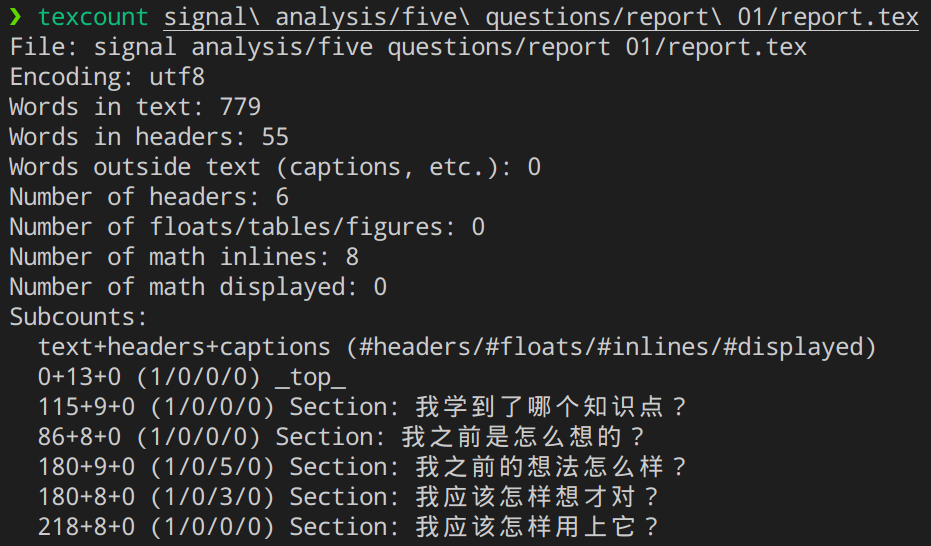
\includegraphics[width=0.9\textwidth]{pics/word count.png}
    \end{center}
\end{document}